% Predicting t9 from t1..t8 -- one forward pass of DTransformer (Algorithm 10)
\documentclass[12pt]{article}
\usepackage[a4paper,margin=2cm]{geometry}
\usepackage{fontspec}
\usepackage{amsmath,amssymb,amsfonts}
\usepackage{booktabs,array}
\usepackage{unicode-math}
\usepackage{booktabs}
\usepackage{xcolor}
\usepackage{nicematrix}
\usepackage{tikz}
\usetikzlibrary{patterns}

\newcommand{\Xt}{\tilde{\symbf{X}}}
\newcommand{\Zt}{\tilde{\symbf{Z}}}
\newcommand{\Wv}{\symbf{W}}

\setmainfont{Libertinus Serif}
\setsansfont{Libertinus Sans}
%\setmonofont{DejaVu Sans Mono}
\setmathfont{STIXTwoMath-Regular.otf}
%\setmathfont{STIX Two Math}

\definecolor{qcol}{HTML}{0B7A83}   % query
\definecolor{kcol}{HTML}{A8630C}   % visible key/value
\definecolor{ksoft}{HTML}{F7E5CB}
\definecolor{offc}{HTML}{E8EBEF}   % masked / zero
\definecolor{hatch}{HTML}{9AA4B2}
\definecolor{mutedc}{HTML}{5A6576}

\setlength{\parindent}{0pt}
\setlength{\parskip}{0.5\baselineskip}


% ------------------------------------------------------------------
% Token row. #1 = query position (1..8); 0 = none highlighted (embedding step);
% 9 = output step (all prompt tokens visible, t9 shown).
% ------------------------------------------------------------------
\newcommand{\tokenrow}[1]{%
\begin{tikzpicture}[x=1cm,y=1cm]
  \foreach \i in {1,...,8}{
    \pgfmathsetmacro{\xx}{(\i-1)*1.08}
    \ifnum#1=0
      \draw[mutedc!40,thick,rounded corners=2pt] (\xx,0) rectangle ++(0.92,0.92);
      \node at (\xx+0.46,0.56) {$t_{\i}$};
    \else\ifnum#1=9
      \draw[kcol,fill=ksoft,thick,rounded corners=2pt] (\xx,0) rectangle ++(0.92,0.92);
      \node at (\xx+0.46,0.56) {$t_{\i}$};
    \else\ifnum\i=#1
      \draw[qcol,fill=qcol,thick,rounded corners=2pt] (\xx,0) rectangle ++(0.92,0.92);
      \node[white] at (\xx+0.46,0.56) {$\symbf{t_{\i}}$};
    \else\ifnum\i<#1
      \draw[kcol,fill=ksoft,thick,rounded corners=2pt] (\xx,0) rectangle ++(0.92,0.92);
      \node at (\xx+0.46,0.56) {$t_{\i}$};
    \else
      \fill[offc,rounded corners=2pt] (\xx,0) rectangle ++(0.92,0.92);
      \fill[pattern=north east lines,pattern color=hatch] (\xx,0) rectangle ++(0.92,0.92);
      \draw[hatch,thick,rounded corners=2pt] (\xx,0) rectangle ++(0.92,0.92);
      \node[mutedc] at (\xx+0.46,0.56) {$t_{\i}$};
    \fi\fi\fi\fi
    \node[font=\tiny,mutedc] at (\xx+0.46,0.2) {pos \i};
    % dashed outline on the token this column predicts
    \pgfmathtruncatemacro{\nx}{#1+1}
    \ifnum\i=\nx \ifnum#1>0 \ifnum#1<8
      \draw[black,very thick,dashed,rounded corners=2pt] (\xx-0.05,-0.05) rectangle ++(1.02,1.02);
    \fi\fi\fi
  }
  % slot 9
  \pgfmathsetmacro{\xx}{8*1.08}
  \ifnum#1>7
    \draw[qcol,very thick,dashed,rounded corners=2pt] (\xx,0) rectangle ++(0.92,0.92);
    \ifnum#1=9 \node[qcol] at (\xx+0.46,0.56) {$\symbf{t_9}$};
    \else \node[qcol] at (\xx+0.46,0.56) {\textbf{?}}; \fi
  \else
    \draw[hatch,thick,dashed,rounded corners=2pt] (\xx,0) rectangle ++(0.92,0.92);
    \node[hatch] at (\xx+0.46,0.56) {?};
  \fi
  \node[font=\tiny,mutedc] at (\xx+0.46,0.2) {pos 9};
\end{tikzpicture}}

\newcommand{\legend}{%
{\small
\tikz\fill[qcol] (0,0) rectangle (0.3,0.3);~query (this column)\quad
\tikz\draw[kcol,fill=ksoft,thick] (0,0) rectangle (0.3,0.3);~visible key/value\quad
\tikz{\fill[offc] (0,0) rectangle (0.3,0.3);\fill[pattern=north east lines,pattern color=hatch] (0,0) rectangle (0.3,0.3);}~masked (future)\quad
\tikz\draw[black,thick,dashed] (0,0) rectangle (0.3,0.3);~token this column predicts}}

% ------------------------------------------------------------------
% Mask matrix, paper layout: rows t_z (keys), columns t_x (queries),
% Mask[t_z,t_x] = [[t_z <= t_x]]. #1 = highlighted query column (0 = none).
% ------------------------------------------------------------------
\newcommand{\maskmatrix}[1]{%
\begin{tikzpicture}[x=0.6cm,y=-0.6cm,font=\small]
  \node[font=\scriptsize,mutedc] at (0.5,0.5) {$z\backslash x$};
  \foreach \c in {1,...,8}{
    \ifnum\c=#1 \node[qcol,font=\small\bfseries] at (\c+0.5,0.5) {\c};
    \else \node[mutedc] at (\c+0.5,0.5) {\c}; \fi }
  \foreach \r in {1,...,8}{
    \node[mutedc] at (0.5,\r+0.5) {\r};
    \foreach \c in {1,...,8}{
      \ifnum\r>\c \def\v{0}\else\def\v{1}\fi
      \ifnum\c=#1
        \ifnum\r=\c
          \fill[qcol] (\c+0.05,\r+0.05) rectangle (\c+0.95,\r+0.95);
          \node[white,font=\small\bfseries] at (\c+0.5,\r+0.5) {1};
        \else\ifnum\v=1
          \draw[kcol,fill=ksoft,thick] (\c+0.05,\r+0.05) rectangle (\c+0.95,\r+0.95);
          \node[font=\small\bfseries] at (\c+0.5,\r+0.5) {1};
        \else
          \fill[offc] (\c+0.05,\r+0.05) rectangle (\c+0.95,\r+0.95);
          \fill[pattern=north east lines,pattern color=hatch] (\c+0.05,\r+0.05) rectangle (\c+0.95,\r+0.95);
          \node[font=\small\bfseries] at (\c+0.5,\r+0.5) {0};
        \fi\fi
      \else
        \ifnum\v=1
          \fill[ksoft!55!offc] (\c+0.05,\r+0.05) rectangle (\c+0.95,\r+0.95);
          \node[mutedc] at (\c+0.5,\r+0.5) {1};
        \else
          \fill[offc] (\c+0.05,\r+0.05) rectangle (\c+0.95,\r+0.95);
          \node[hatch] at (\c+0.5,\r+0.5) {0};
        \fi
      \fi
    }}
\end{tikzpicture}}

% Same mask in the GPT-2 code layout: rows i (queries), columns j (keys), 0-indexed.
% m[i,j] = [[ i >= j - ns + nd ]], which is i >= j when nd = ns = 8. #1 = highlighted token (1..8).
\newcommand{\maskmatrixcode}[1]{%
\begin{tikzpicture}[x=0.6cm,y=-0.6cm,font=\small]
  \node[font=\scriptsize,mutedc] at (0.5,0.5) {$i\backslash j$};
  \foreach \c in {1,...,8}{
    \pgfmathtruncatemacro{\cl}{\c-1}
    \node[mutedc] at (\c+0.5,0.5) {\cl}; }
  \foreach \r in {1,...,8}{
    \pgfmathtruncatemacro{\rl}{\r-1}
    \ifnum\r=#1 \node[qcol,font=\small\bfseries] at (0.5,\r+0.5) {\rl};
    \else \node[mutedc] at (0.5,\r+0.5) {\rl}; \fi
    \foreach \c in {1,...,8}{
      \ifnum\c>\r \def\v{0}\else\def\v{1}\fi
      \ifnum\r=#1
        \ifnum\r=\c
          \fill[qcol] (\c+0.05,\r+0.05) rectangle (\c+0.95,\r+0.95);
          \node[white,font=\small\bfseries] at (\c+0.5,\r+0.5) {1};
        \else\ifnum\v=1
          \draw[kcol,fill=ksoft,thick] (\c+0.05,\r+0.05) rectangle (\c+0.95,\r+0.95);
          \node[font=\small\bfseries] at (\c+0.5,\r+0.5) {1};
        \else
          \fill[offc] (\c+0.05,\r+0.05) rectangle (\c+0.95,\r+0.95);
          \fill[pattern=north east lines,pattern color=hatch] (\c+0.05,\r+0.05) rectangle (\c+0.95,\r+0.95);
          \node[font=\small\bfseries] at (\c+0.5,\r+0.5) {0};
        \fi\fi
      \else
        \ifnum\v=1
          \fill[ksoft!55!offc] (\c+0.05,\r+0.05) rectangle (\c+0.95,\r+0.95);
          \node[mutedc] at (\c+0.5,\r+0.5) {1};
        \else
          \fill[offc] (\c+0.05,\r+0.05) rectangle (\c+0.95,\r+0.95);
          \node[hatch] at (\c+0.5,\r+0.5) {0};
        \fi
      \fi
    }}
\end{tikzpicture}}

% Which columns of W_p are read: 8 of 1024
\newcommand{\wpbar}{%
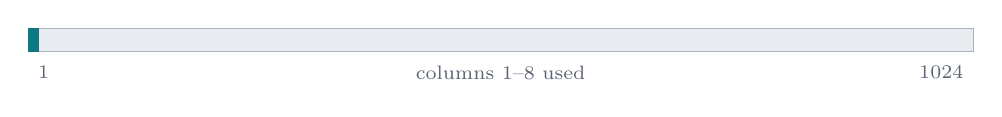
\begin{tikzpicture}
  \draw[mutedc!50,fill=offc] (0,0) rectangle (12,0.3);
  \fill[qcol] (0,0) rectangle (0.14,0.3); % 8/1024 of 12cm is 0.094cm; widened slightly to stay visible
  \node[font=\scriptsize,mutedc,anchor=north west] at (0,-0.05) {1};
  \node[font=\scriptsize,mutedc,anchor=north] at (6,-0.05) {columns 1--8 used};
  \node[font=\scriptsize,mutedc,anchor=north east] at (12,-0.05) {1024};
\end{tikzpicture}}

% ------------------------------------------------------------------
% One query-column step. #1 = t_x in 1..8
% ------------------------------------------------------------------
\newcommand{\querystep}[1]{%
  \edef\tn{\the\numexpr#1+1\relax}%
  \subsection*{Line 6, query column $t_x=#1$ of 8: which tokens can $t_{#1}$ see?}
  \tokenrow{#1}\par
  \noindent
  \begin{minipage}[t]{0.40\linewidth}\vspace{0pt}
    \maskmatrix{#1}\par
    {\small\color{mutedc} Column $t_x=#1$: \ifnum#1=1 row 1 is\else rows 1--#1 are\fi{} 1%
    \ifnum#1<8; \ifnum#1=7 row 8 gets\else rows \tn--8 get\fi{} $S=-\infty$ before the softmax\else; no row is masked\fi.}
  \end{minipage}\hfill
  \begin{minipage}[t]{0.56\linewidth}\vspace{0pt}
    \small
    \begin{tabular}{@{}ll@{}}
      \toprule
      $\ell_x$ (queries) & $8$\\
      $\ell_z$ (keys, values) & $8$\\
      $\Xt=\Zt$ & $768\times 8$\\
      Per head: $\symbf{Q},\symbf{K},\symbf{V}$ & $64\times 8$ each\\
      $\symbf{S}=\symbf{K}^{\top}\symbf{Q}$ & $8\times 8$ \ ($\ell_z\times\ell_x$)\\
      \midrule
      Query column viewed & \textcolor{qcol}{$t_x=#1$}\\
      Keys it can see & \textcolor{qcol}{\ifnum#1=1 $t_z=1$ (itself only)\else $t_z=1,\dots,#1$ \ (#1 of 8)\fi}\\
      Masked keys & \ifnum#1<8 \ifnum#1=7 $t_z=8$\else $t_z=\tn,\dots,8$\fi\else none\fi\\
      $\symbf{P}[:,#1]$ estimates & $\hat{P}(x[\tn]\mid x[1{:}#1])$\\
      Is $x[\tn]$ already known? & \ifnum#1<8 yes: $t_{\tn}$\else \textcolor{qcol}{no: this is $t_9$}\fi\\
      \bottomrule
    \end{tabular}
  \end{minipage}

  \ifnum#1=1
  All eight query columns are computed at once, in one matrix product per head.
  Going through them one at a time is only a way to read the mask.
  \par\fi
  Query $t_x=#1$ is $t_{#1}$. The mask keeps keys with $t_z\le #1$, so
  \ifnum#1=1 it can attend only to itself\else it attends to $t_1,\dots,t_{#1}$\fi
  \ifnum#1<8 \ifnum#1=7 \space and never sees $t_8$\else\space and never sees $t_{\tn},\dots,t_8$\fi\else, the whole prompt\fi.

  Because this holds in every layer, column $#1$ of the output depends only on $x[1{:}#1]$.
  So $\symbf{P}[:,#1]$ is a prediction of $x[\tn]$.

  \ifnum#1<8
  But $x[\tn]=t_{\tn}$ is already in the prompt. At inference this column is computed and thrown away.
  In training it is one of the 8 loss terms.
  \else
  $x[9]$ is not in the prompt. This is the only column inference needs:
  $\symbf{P}[:,8]=\hat{P}(x[9]\mid t_1,\dots,t_8)$.
  \fi
  \par\bigskip
}

\title{Formal Algorithms for GPT-2 Small Model\\[4pt]
        \Large{Predicting $t_9$ from $t_1,\dots,t_8$} \\[4pt]
        \large{One Forward Pass of DTransformer --- Algorithm 10}}
\author{Devi Prasad M}
\date{September, 2026}

\begin{document}
\maketitle

\section*{Setup}

The prompt is $x=(t_1,\dots,t_8)$, so $\ell=\operatorname{length}(x)=8$.
We follow one call of Algorithm 10 and read the causal mask one query position at a time.

\begin{center}
\begin{tabular}{@{}llll@{}}
  \toprule
  $\ell$ & $8$ & $d_e, d_{in}, d_{out}$ & $768$\\
  $\ell_{\max}$ & $1024$ & $H$ & $12$\\
  $L$ & $12$ & $d_{\text{attn}},d_{\text{mid}}$ & $64$\\
  $N_V$ & $50257$ & $d_{\text{mlp}}$ & $3072$\\
  \bottomrule
\end{tabular}
\end{center}

\textbf{Notation.} The paper prints line 6 of Algorithm 10 as
$\operatorname{MHAttention}(\Xt\mid\mathcal{W}_l,\text{Mask})$.
Algorithm 5 takes two sequences, so we write the call in full as
$\operatorname{MHAttention}(\Xt,\Xt\mid\mathcal{W}_l,\text{Mask})$: in self-attention the context $\Zt$ is $\Xt$ itself.

\textbf{Mask convention.} As in the paper, $\text{Mask}\in\{0,1\}^{\ell_z\times\ell_x}$: rows are key positions $t_z$,
columns are query positions $t_x$, and $\text{softmax}$ runs down each column of $\symbf{S}$.

\legend

% ------------------------------------------------------------------
\subsection*{Line 2, embeddings: build $\symbf{X}$ from 8 tokens and 8 positions}

\begin{center}
\fbox{\small $2\quad \text{for } t\in[\ell]:\ \symbf{e}_t\leftarrow \Wv_{\symbf{e}}[:,x[t]]+\Wv_{\symbf{p}}[:,t]$}
\end{center}

\tokenrow{0}

\begin{center}
\small
\begin{tabular}{@{}ll@{}}
  \toprule
  $\ell\leftarrow\operatorname{length}(x)$ & $8$\\
  Token columns read & $\Wv_{\symbf{e}}[:,x[1]],\dots,\Wv_{\symbf{e}}[:,x[8]]$\\
  Position columns read & $\Wv_{\symbf{p}}[:,1{:}8]$ \ (8 of 1024)\\
  $\symbf{e}_t$ & $768\times 1$ each\\
  $\symbf{X}=[\symbf{e}_1,\dots,\symbf{e}_8]$ & $768\times 8$\\
  Padding to $\ell_{\max}$ & none\\
  \bottomrule
\end{tabular}
\end{center}

Position embedding columns read from $\Wv_{\symbf{p}}\in\mathbb{R}^{768\times 1024}$:\par
\wpbar

All eight tokens go in together. Each gets its token embedding plus the position embedding for its slot.
Only columns 1--8 of $\Wv_{\symbf{p}}$ are read. $\ell_{\max}=1024$ is the number of columns $\Wv_{\symbf{p}}$ has,
the longest input the model accepts. Nothing is padded to 1024.

From here on every layer works on $\symbf{X}\in\mathbb{R}^{768\times 8}$, so every attention call has $\ell_x=\ell_z=8$.

\bigskip
% ------------------------------------------------------------------
\begin{center}
\fbox{\small $6\quad \symbf{X}\leftarrow\symbf{X}+\operatorname{MHAttention}\bigl(\Xt,\Xt\mid\mathcal{W}_l,\ \text{Mask}[t_z,t_x]=[[t_z\le t_x]]\bigr)$}\par
{\small\color{mutedc} Runs in each of the $L=12$ layers.}
\end{center}

\querystep{1}
\querystep{2}
\querystep{3}
% Steps 4--6 follow the same pattern. Uncomment to include them.
% \querystep{4}
% \querystep{5}
% \querystep{6}
\begin{center}\large$\vdots$\end{center}
\querystep{7}
\querystep{8}

% ------------------------------------------------------------------
\subsection*{Line 11, output: sample $t_9$ from column 8 of $\symbf{P}$}

\begin{center}
\fbox{\small $11\quad \text{return } \symbf{P}=\operatorname{softmax}(\Wv_{\symbf{u}}\symbf{X})$}\par
{\small\color{mutedc} Then Algorithm 14, line 4 with $i=1$: $\symbf{p}\leftarrow\symbf{P}[:,\ell+i-1]=\symbf{P}[:,8]$.}
\end{center}

\tokenrow{9}

\begin{center}
\small
\begin{tabular}{@{}ll@{}}
  \toprule
  $\symbf{X}$ after final layer norm & $768\times 8$\\
  $\Wv_{\symbf{u}}$ & $50257\times 768$\\
  $\symbf{P}=\operatorname{softmax}(\Wv_{\symbf{u}}\symbf{X})$ & $50257\times 8$\\
  Columns 1--7 & computed, not used at inference\\
  Column used & \textcolor{qcol}{$\symbf{P}[:,8]=\hat{P}(x[9]\mid x[1{:}8])$}\\
  Sample & \textcolor{qcol}{$t_9\sim\symbf{q}\propto\symbf{P}[:,8]^{1/\tau}$}\\
  \bottomrule
\end{tabular}
\end{center}

$\symbf{P}$ has one column per input position. Column $t$ is the model's distribution over the next token after $x[1{:}t]$.

At inference only the last column matters. Columns 1--7 predict tokens we already have, $t_2,\dots,t_8$.

In training, the same pass is used differently: all 8 columns are scored against their known next tokens,
giving 8 loss terms from one forward pass. The causal mask is what makes that valid.

% ------------------------------------------------------------------
\subsection*{Appendix: the same mask in the GPT-2 code}

The openai/gpt-2 code (\texttt{src/model.py}) stores the mask transposed: rows are queries $i$ (destination),
columns are keys $j$ (source), both 0-indexed. \texttt{attention\_mask(nd, ns)} sets
\[
  m[i,j] = [[\, i \ge j - n_s + n_d \,]],
\]
which is $i\ge j$ when $n_d=n_s=8$. The softmax runs along each row. Below, token $t_3$ (row $i=2$) is highlighted;
compare with the paper-layout matrix at $t_x=3$.

\begin{center}
\maskmatrixcode{3}
\end{center}


\section*{An eight-token prompt.}
Let
\[
\mathbf{x}=(t_1,t_2,\ldots,t_8), \qquad
\ell_x=\operatorname{length}(\mathbf{x})=8.
\]
A call to \(P=\operatorname{DTransformer}(\mathbf{x}\mid\hat\theta)\)
produces eight output columns. Column \(P[:,j]\) gives a distribution
for the token \emph{after} the prefix \((t_1,\ldots,t_j)\).

\begin{center}
\renewcommand{\arraystretch}{1.25}
\begin{tabular}{@{}c>{$}l<{$}>{$}l<{$}>{$}l<{$}@{}}
\toprule
Position \(j\) &
\multicolumn{1}{c}{Initial column \(X^{(0)}[:,j]\)} &
\multicolumn{1}{c}{Visible positions} &
\multicolumn{1}{c}{Next-token distribution} \\
\midrule
1 & W_e[:,t_1]+W_p[:,1] & \{1\}       & P[:,1] \\
2 & W_e[:,t_2]+W_p[:,2] & \{1,2\}     & P[:,2] \\
3 & W_e[:,t_3]+W_p[:,3] & \{1,2,3\}   & P[:,3] \\
\multicolumn{4}{c}{$\vdots$} \\
7 & W_e[:,t_7]+W_p[:,7] & \{1,\ldots,7\} & P[:,7] \\
8 & W_e[:,t_8]+W_p[:,8] & \{1,\ldots,8\} & P[:,8] \\
\bottomrule
\end{tabular}
\end{center}

\section*{The causal attention mask.}
Rows index a potential source (context) position \(r\); columns index
the position \(j\) whose representation is being updated:
\[
    \operatorname{Mask}[r,j] =
        \begin{cases}
        1, & r\leq j,\\
        0, & r>j.
        \end{cases}
\]
For this prompt, the complete mask is
\[
\begin{array}{c@{\quad}c}
&
\begin{array}{cccccccc}
\scriptstyle j=1&\scriptstyle 2&\scriptstyle 3&\scriptstyle 4&
\scriptstyle 5&\scriptstyle 6&\scriptstyle 7&\scriptstyle 8
\end{array}
\\[-2pt]
\begin{array}{c}
\scriptstyle r=1\\[-1pt]\scriptstyle 2\\[-1pt]\scriptstyle 3\\[-1pt]
\scriptstyle 4\\[-1pt]\scriptstyle 5\\[-1pt]\scriptstyle 6\\[-1pt]
\scriptstyle 7\\[-1pt]\scriptstyle 8
\end{array}
&
\left[
\begin{array}{cccccccc}
1&1&1&1&1&1&1&1\\
0&1&1&1&1&1&1&1\\
0&0&1&1&1&1&1&1\\
0&0&0&1&1&1&1&1\\
0&0&0&0&1&1&1&1\\
0&0&0&0&0&1&1&1\\
0&0&0&0&0&0&1&1\\
0&0&0&0&0&0&0&1
\end{array}
\right]
\end{array}
\]
Thus column \(j=3\) can attend only to positions \(1,2,3\), whereas
column \(j=8\) can attend to all eight positions. A zero forbids an
attention link; it does not replace an input token.

\paragraph{Predicting \(t_9\).}
After all transformer layers and the final unembedding, Algorithm~14
takes
\[
\mathbf{p}=P[:,\ell_x]=P[:,8]
 =\widehat{\Pr}_{\hat\theta}
   \bigl(\,\cdot\mid t_1,\ldots,t_8\bigr).
\]
The next token \(t_9\) is selected or sampled from this distribution.
There is no \(t_9\) input column in this forward pass.
\end{document}
